\documentclass[tikz, border=1mm]{standalone}
\usepackage{tikz} 
\usetikzlibrary{arrows.meta}
\usepackage{pgfplots}

\begin{document}

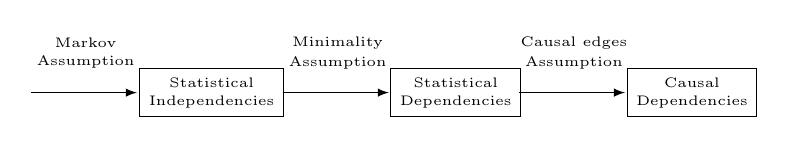
\begin{tikzpicture}
    % nodes
    \node at (-3.7,0.5) {\tiny{\shortstack{Markov \\ Assumption}}};
    \node at (-2.1,0) [rectangle,draw]  {\tiny{\shortstack{Statistical \\ Independencies}}};
    \node at (-0.5,0.5) {\tiny{\shortstack{Minimality \\ Assumption}}};
    \node at (1,0) [rectangle,draw]  {\tiny{\shortstack{Statistical \\ Dependencies}}};
    \node at (2.5,0.5) {\tiny{\shortstack{Causal edges \\ Assumption}}};
    \node at (4,0) [rectangle,draw]  {\tiny{\shortstack{Causal \\ Dependencies}}};
	
    % paths
    \draw[-{latex}](-4.4,0) to (-3.05,0);
    \draw[-{latex}](-1.2,0) to (0.15,0);
    \draw[-{latex}](1.8,0) to (3.15,0);
\end{tikzpicture}
  
\end{document}
